\documentclass{standalone}
\usepackage{tikz}
\usetikzlibrary{positioning,calc,patterns,decorations.pathmorphing}

\begin{document}

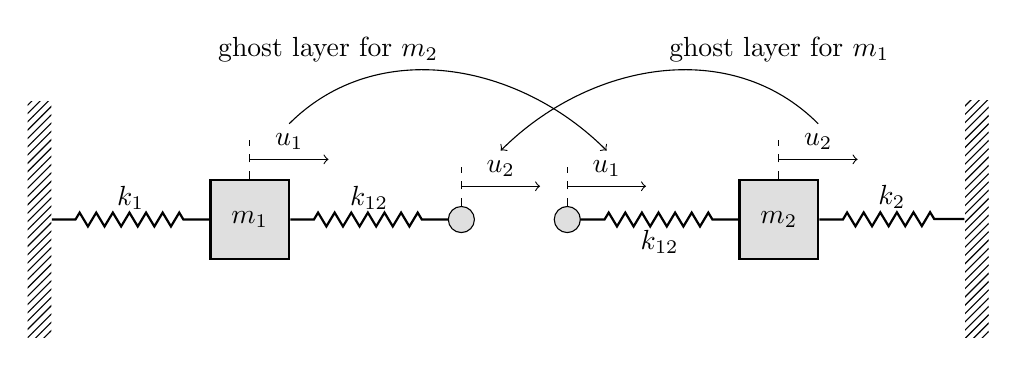
\begin{tikzpicture}
    \tikzstyle{spring}=[thick,decorate,decoration={zigzag,pre length=0.3cm,post length=0.3cm,segment length=6}]
    \tikzstyle{ground}=[fill,pattern=north east lines,draw=none,minimum width=0.75cm,minimum height=0.3cm]
    \tikzstyle{mass}=[draw, fill=gray!25, thick, minimum width=1cm, minimum height=1cm]
    \node (W1) [ground, rotate=-90, minimum width=3cm] {};
    \node (M1) [mass, right= 2cm of W1.north] {$m_1$};
    \node (M2fake) [circle, draw=black, fill=gray!25, right= 2cm of M1] {};

    \draw [dashed] (M2fake.north) -- ++ (0,.5);
    \draw [->] ($(M2fake.north) + (0,.25)$) -- node[above](U2ToM1){$u_2$} ++ (1,0);
    \draw [dashed] (M1.north) -- ++ (0,.5);
    \draw [->] ($(M1.north) + (0,.25)$) -- node[above](U1FromM1){$u_1$} ++ (1,0);
    \draw [spring] (W1.north) -- node[above]{$k_1$}(M1.west);
    \draw [spring] (M1.east) -- node[above]{$k_{12}$}(M2fake.west);

    \node (M1fake) [circle, draw=black, fill=gray!25, right= 1cm of M2fake] {};
    \node (M2) [mass, right= 2cm of M1fake] {$m_2$};
    \draw [dashed] (M2.north) -- ++ (0,.5);
    \draw [->] ($(M2.north) + (0,.25)$) -- node[above](U2FromM2){$u_2$} ++ (1,0);
    \draw [dashed] (M1fake.north) -- ++ (0,.5);
    \draw [->] ($(M1fake.north) + (0,.25)$) -- node[above](U1ToM2){$u_1$} ++ (1,0);

    \node (W2) [ground, rotate=90, minimum width=3cm, right= 2cm of M2, xshift=-1.5cm] {};
    \draw [spring] (M2.east) -- node[above]{$k_2$}(W2.north);
    \draw [spring] (M1fake.east) -- node[below]{$k_{12}$}(M2.west);

    \draw[](U2FromM2.north) edge[->,out=135, in=45] node[above right]{ghost layer for $m_1$} (U2ToM1.north);
    \draw[](U1FromM1.north) edge[->,out=45, in=135] node[above left]{ghost layer for $m_2$} (U1ToM2.north);

\end{tikzpicture}
\end{document}
